%&pdflatex
\documentclass[11pt, a4paper]{article}
\usepackage{graphicx}
\usepackage{amsmath}
\usepackage{listings}
\usepackage{minted}
\usepackage{physics}
\usepackage{hyperref}
\hypersetup{
    colorlinks=true, %set true if you want colored links
    linktoc=all,     %set to all if you want both sections and subsections linked
    linkcolor=magenta,  %choose some color if you want links to stand out
}

\title{\textbf{EE2703 Applied Programming Lab - Assignment No 7}}
\author{
  \textbf{Name}: Abishek S\\
  \textbf{Roll Number}: EE18B001
}\date{\today}
\begin{document}
		
\maketitle 
\section{Abstract}
The goal of this assignment is the following :
\begin{itemize}
\item To understand and use symbolic python for analysing Laplace equations and solving them.
\item To realise low pass and high pass filters using opamp circuits.
\item To plot graphs and observe the output of low pass and high pass filters to different inputs.
\end{itemize}
\usemintedstyle{manni}

\section{Assignment}
\subsection{Setting up the Program}
Importing the standard libraries
\begin{minted}[mathescape,escapeinside = ||,obeytabs,tabsize = 4]{python3}
import pylab as pl
import numpy as np
import sys
import scipy.signal as sp
import matplotlib
from sympy import *
\end{minted}

We initialize sympy and define utility functions for general plotting and making Bode plots..
\begin{minted}[obeytabs,tabsize = 4]{python3}
init_printing()
#Complex variable of Laplace equations
s = symbols('s')

#Defining a general utility function PLOT for plotting
def PLOT(x,y,fig_no = 0,label_x = r'$\rightarrow$',
	label_y = r'$\rightarrow$',fn = pl.plot,arg3 = 'b-',
	title = "Plot",grids = True,cmap = matplotlib.cm.jet,label = ''):
	'''Plotting function to make standard plots'''
	pl.figure(fig_no)
	pl.grid(grids)
	if fn == pl.contourf:
		fn(x,y,arg3,cmap = cmap)
		pl.colorbar()
	else:
		if label == '':
			fn(x,y,arg3)
		else:
			fn(x,y,arg3,label = label)
			pl.legend()
	pl.xlabel(label_x,size = 17)
	pl.ylabel(label_y,size = 17)
	pl.title(title)

#Defining a general utility function for making BODE Plots
def bodeplot(H,fig_no = 0,title = ''):
	'''Makes Bode Plots'''
	pl.figure(fig_no)
	pl.suptitle(title)
	w,s,phi = H.bode()
	pl.subplot(2,1,1)
	pl.semilogx(w,s)
	pl.xlabel(r'$\omega$',size=17)
	pl.ylabel(r'$|H(j\omega)|-(in dB)$',size =17)
	pl.subplot(2,1,2)
	pl.semilogx(w,phi)
	pl.xlabel(r'$\omega$',size=17)
	pl.ylabel(r'$\angle(H(j\omega))$',size =17)
	
\end{minted}

\subsection{Low Pass Filter}
{
We analyse the given circuit for Butterworth low pass filter and obtain the equations in a matrix form for solving.
}
\[\begin{pmatrix} 0 & 0 & 1 & -\frac{1}{G} 
\\ -\frac{1}{1+sR2C2} & 1 & 0 & 0 
\\ 0 & -G & G & 1 
\\ -\frac{1}{R_1}-\frac{1}{R_2}-sC_1 & \frac{1}{R2} & 0 & sC_1 
\end{pmatrix}
\begin{pmatrix} V_1 \\ V_p \\ V_m \\ V_o \end{pmatrix}
 = 
\begin{pmatrix} 0 \\ 0 \\ 0 \\ -V_i(s)/R_1 \end{pmatrix}\]

We obtain the output voltage in symolic form by solving the above matrix equation.
\begin{minted}[obeytabs,tabsize = 4]{python3}
#Solving the matrix equation and getting the output Voltage for Low Pass Filter
def LowPass(R1,R2,C1,C2,G,Vi=1):
    '''Active 2nd order low pass butterworth filter using opamp''' 
    A = Matrix([[0,0,1,-1/G],[-1/(1+s*R2*C2),1,0,0],
    		[0,-G,G,1],[-1/R1-1/R2-s*C1,1/R2,0,s*C1]])
    b = Matrix([0,0,0,-Vi/R1])
    V = A.inv()*b
    return(A,b,V)
    
\end{minted}

We also define two functions to obtain the transfer function in sp.lti form from the symbolic form obtained by solving the matrix equations.
\begin{minted}[obeytabs,tabsize = 4]{python3}
#Extract the Transfer function and convert it to scipy lti form
def Simplify_H(V):
    '''Extracts Transfer function from the matrix inversion result'''
    Vo = V[3]  #The third element in the V column is the output voltage
    Vo = expand(simplify(Vo))  #converting to rational form
    H = SympyToScipy(Vo)
    return H

#Convert the Transfer function form sympy to scipy lti form
def SympyToScipy(Vo):
    '''Converts Transfer function in sympy to scipy'''
    v1 = fraction(Vo) #converting to numerator and denominator form
    n,d = Poly(v1[0],s),poly(v1[1],s)
    numer,denom = n.all_coeffs(), d.all_coeffs()  #extract the coefficients of 's'
    numer,denom = [float(f) for f in numer], [float(f) for f in denom]
    H = sp.lti(numer,denom)  #converting to scipy lti form
    return H
    
\end{minted}

We get the Transfer function and make the bode plot for Low Pass Filter.
\begin{minted}[obeytabs,tabsize = 4]{python3}
#Values of R1,R2,C1,C2,G chosen from given circuit
A,b,V = LowPass(10000,10000,1e-9,1e-9,1.586,1)
H_lp = Simplify_H(V)

bodeplot(H_lp,1,"Bode plot of Low Pass Filter")
pl.show()

\end{minted}

\begin{figure}[H]
   	\centering
   	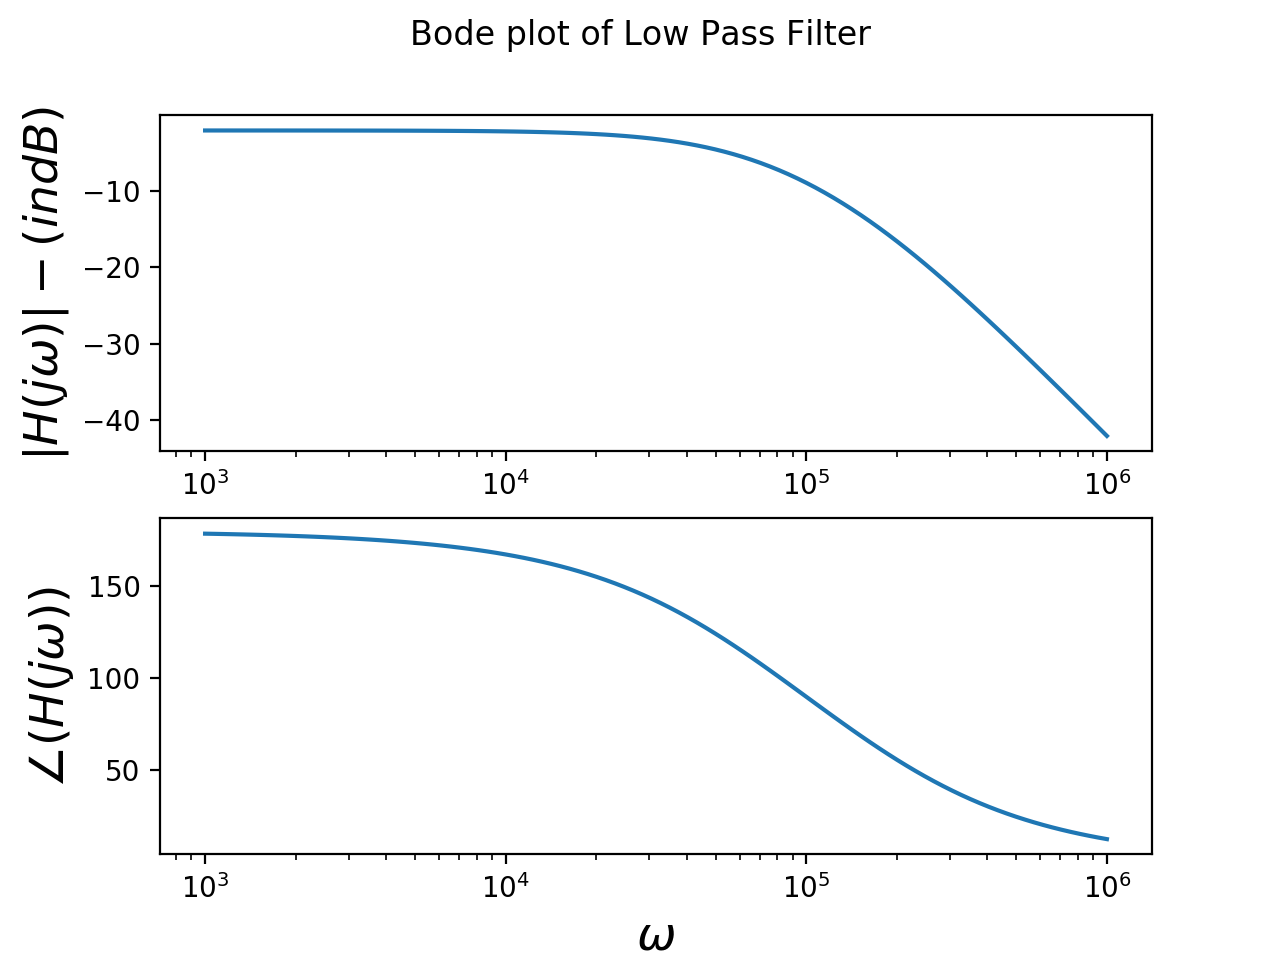
\includegraphics[scale=0.8]{bode_lpf.png}
   	\label{fig:bode_lpf}
   	\caption{Bode Plot for Low Pass Filter}
\end{figure}

\subsection{High Pass Filter}
{
We analyse the given circuit for high pass filter and obtain the equations in a matrix form for solving.
}
\[\begin{pmatrix} 0 & 0 & 1 & -\frac{1}{G} 
\\ -\frac{-sR_3C_2}{1+sR_3C_2} & 1 & 0 & 0 
\\ 0 & -G & G & 1 
\\ -1-(sR_1C_1)-(sR_3C_2)) & sC_2R_1 & 0 & 1 
\end{pmatrix}
\begin{pmatrix} V_1 \\ V_p \\ V_m \\ V_o \end{pmatrix} 
= 
\begin{pmatrix} 0 \\ 0 \\ 0 \\ -V_i(s)sR_1C_1 \end{pmatrix}\]


We obtain the output voltage in symolic by solving the above matrix equation.
\begin{minted}[obeytabs,tabsize = 4]{python3}
#Solving the matrix equation and getting the output Voltage for High Pass Filter
def HighPass(R1,R2,C1,C2,G,Vi = 1):
    '''Active 2nd order high pass filter using opamp'''
    A = Matrix([[0,0,1,-1/G],[-1/(1+1/(s*R2*C2)),1,0,0],
    		[0,-G,G,1],[-s*C1-s*C2-1/R1,s*C2,0,1/R1]])
    b = Matrix([0,0,0,-Vi*s*C1])
    V = A.inv()*b
    return(A,b,V)
\end{minted}

\hypertarget{hpf}
We get the Transfer function and make the bode plot for High Pass Filter.
\begin{minted}[obeytabs,tabsize = 4]{python3}
#Values of R1,R2,C1,C2,G chosen from given circuit
A,b,V = HighPass(1e4,1e4,1e-9,1e-9,1.586,1)
H_hp = Simplify_H(V)

bodeplot(H_hp,2,"Bode plot of High Pass Filter")
pl.show()

\end{minted}

\begin{figure}[H]
   	\centering
   	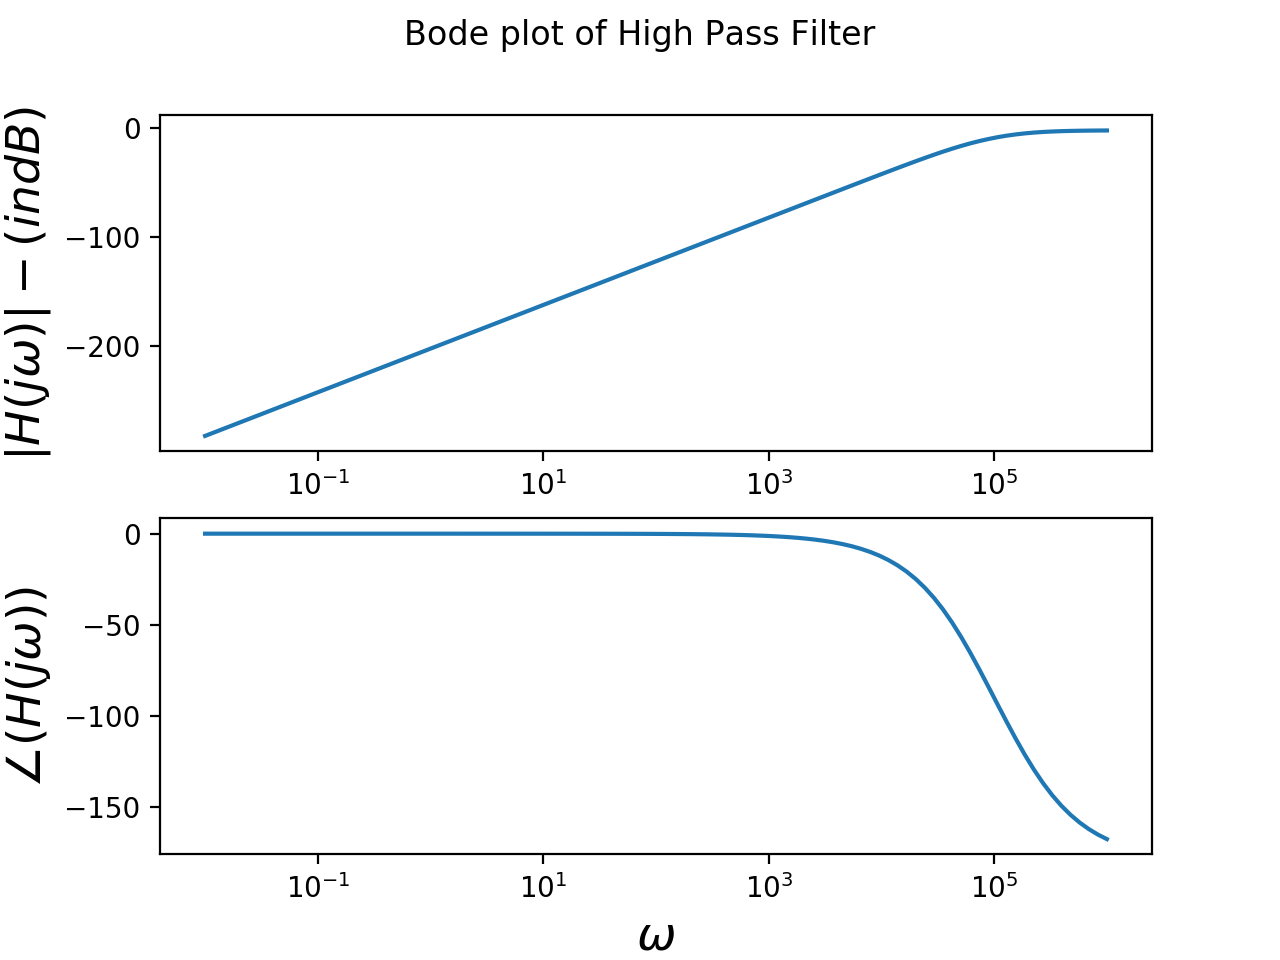
\includegraphics[scale=0.8]{bode_hpf.png}
   	\label{fig:bode_hpf}
   	\caption{Bode Plot for High Pass Filter}
\end{figure}
{
We observe that the Transfer function of the \textbf{low pass filter drops off towards higher frequencies} and that of the \textbf{high pass filter increases towards higher frequencies}, hence their names.
}

\section{Assignment Questions}
\subsection{Question 1}
{
We plot the \textbf{step response} of Low Pass Filter, (i.e) output of low pass filter for input :
\(v_i(t) = u(t)\)
which implies $V_i(S) = 1/S$.
}
\begin{minted}[obeytabs,tabsize = 4]{python3}
t = np.arange(0,1e-2,1e-7)  #Time scale

A,b,V = LowPass(10000,10000,1e-9,1e-9,1.586,1/s)
_,vtd = sp.impulse(Simplify_H(V),None,t)
PLOT(t,vtd,3,r"$t$",r'$V_o(t)$',pl.plot,
	title = 'Step response of Low Pass Filter')
pl.show()

\end{minted}
\begin{figure}[H]
   	\centering
   	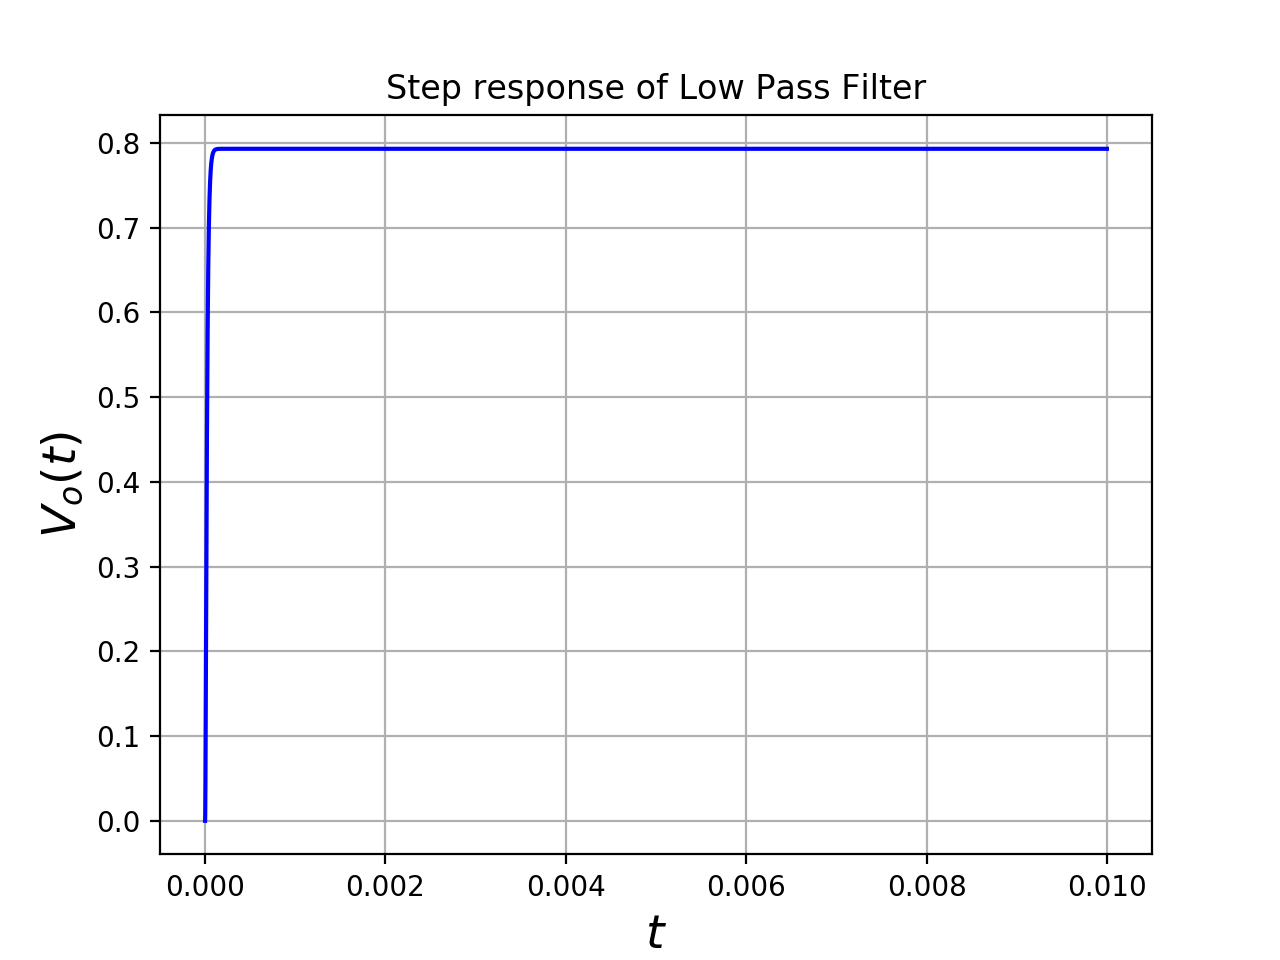
\includegraphics[scale=0.5]{step_lpf.png}
   	\label{fig:step_lpf}
   	\caption{Response of Low pass Filter to unit step function}
\end{figure}
{ 
We observe that the step response of the low pass filter \textbf{starts from zero initially} when the input suddenly changes at t = 0 as it doesn't allow the high frequency.
\\Then it settles to a final value of 0.79 as it \textbf{allows DC input intact} due to it's low frequency.
\\\textbf{No overshoot} in low pass filter case as it is a Butterworth filter.
}

\subsection{Question 2}
{
We plot the input voltage which is \textbf{sum of two sinusoids} of different frequencies. We also plot the \textbf{response of Low pass Filter} to the input.
}
The input voltage is given as :
\[v_i(t) = (\sin(2000\pi t) + cos(2 \times 10^6\pi t))u(t)\]
\begin{minted}[obeytabs,tabsize = 4]{python3}
t = np.arange(0,5e-3,1e-7)  #Time scale

inp = np.sin(2000*np.pi*t)+np.cos(2*(10**6)*np.pi*t)
PLOT(t,inp,5,r'$t$',r'$V_i(t)$',title = 'Sum of 2 sinusoids Input')
pl.show()

\end{minted}
\begin{figure}[H]
   	\centering
   	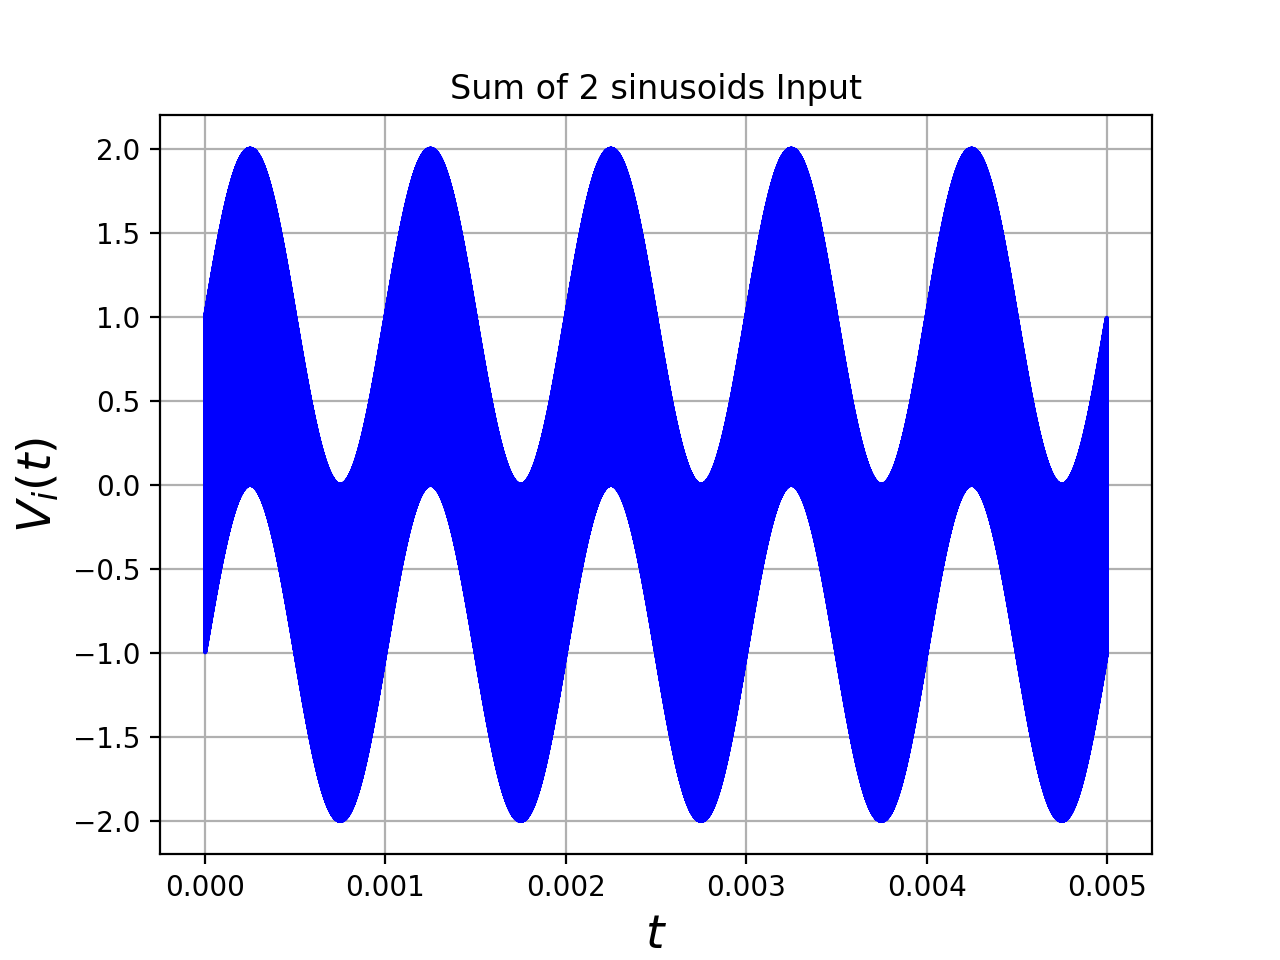
\includegraphics[scale=0.5]{vi_2.png}
   	\label{fig:vi_2}
   	\caption{Input voltage comprising of sum of two sinusoids}
\end{figure}
\begin{minted}[obeytabs,tabsize = 4]{python3}
t,vtd,svec = sp.lsim(H_lp,inp,t)
PLOT(t,vtd,6,r"$t$",r'$V_o(t)$',pl.plot,
	title = 'Response of low pass filter to sum of 2 sinusoids')
pl.show()

\end{minted}
\begin{figure}[H]
   	\centering
   	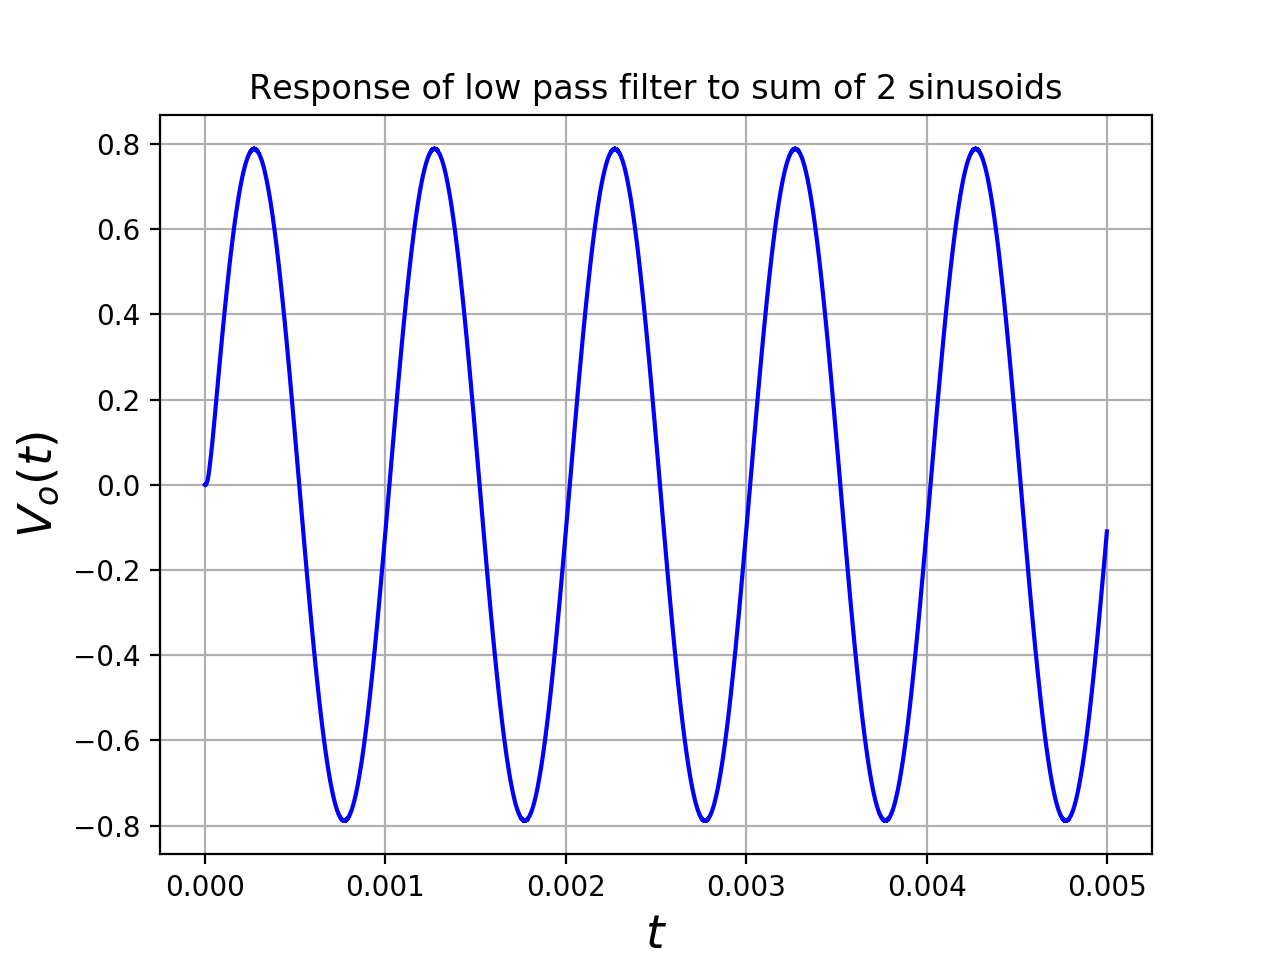
\includegraphics[scale=0.5]{lpf_2.png}
   	\label{fig:lpf_2}
   	\caption{Response of Low pass Filter to sum of two sinusoids}
\end{figure}
{
As expected low pass filter \textbf{allows the low frequency sinusoid} to pass intact, and \textbf{blocks the high frequency sinusoid} almost completely.
}

\subsection{Question 3}
{
Refer \hyperlink{hpf}{this figure} for the Bode Plot of High Pass Filter.
We plot the response of the high pass filter to a \textbf{sum of two input sinusoids}.
}
\begin{minted}[obeytabs,tabsize = 4]{python3}
t = np.arange(0,1e-5,1e-7)  #Time scale

inp = np.sin(2000*np.pi*t)+np.cos(2*(10**6)*np.pi*t)
t,vtd,svec = sp.lsim(H_hp,inp,t)
PLOT(t,vtd,7,r"$t$",r'$V_o(t)$',pl.plot,
	title = 'Response of high pass filter to sum of 2 sinusoids')
pl.show()

\end{minted}
\begin{figure}[H]
   	\centering
   	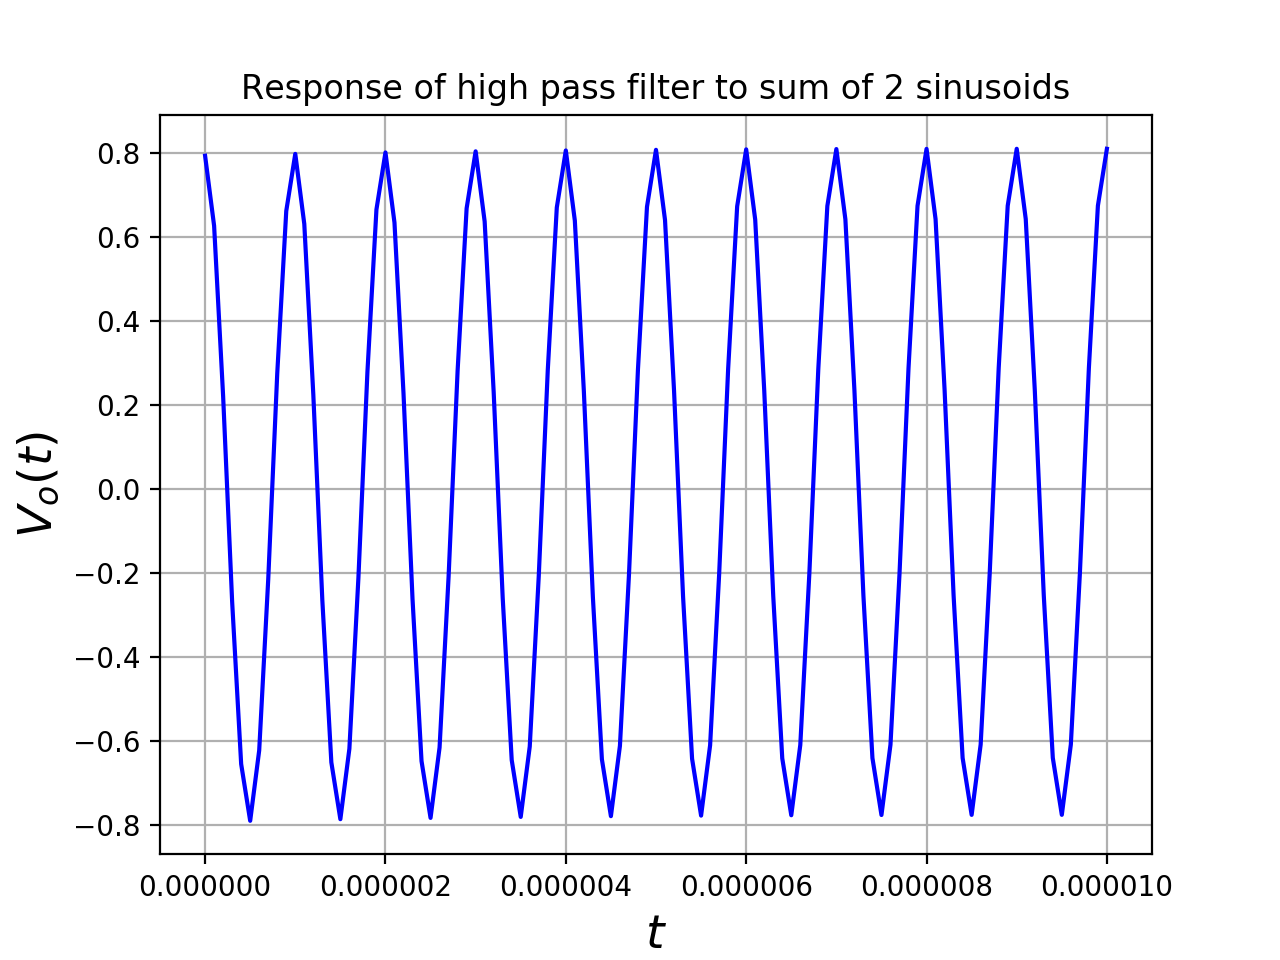
\includegraphics[scale=0.5]{hpf_2.png}
   	\label{fig:hpf_2}
   	\caption{Response of High pass Filter to sum of two sinusoids}
\end{figure}
{
High pass filter \textbf{allows the high frequency sinusoid} to pass intact, and \textbf{blocks the low frequency sinusoid} almost completely.
\\We have used different time scales on both plots to capture the responses better.
}

\subsection{Question 4}
{
We \textbf{input damped sinusoidal inputs} of low and high frequencies to both the circuits and observe how they respond. We use different time scales for both frequencies and different damping to observe the variations better.
}
\subsubsection{High Frequency Damped sinusoid}
{
The first input voltage is given as :
\[v_i(t) = (\cos(10^6 t) \times e^{-3000t})u(t)\]
}
\begin{minted}[obeytabs,tabsize = 4]{python3}
#Response of Low Pass and High Pass filter to high frequency damped sinusoid
damping_factor = 3000

t = np.arange(0,5e-4,1e-7)  #Time scale

inp = np.exp(-damping_factor*t)*(np.cos((10**6)*np.pi*t))
PLOT(t,inp,8,r'$t$',r'$V_i(t)$',title = 'High Frequency damped sinusoid input')
pl.show()

t,vtd,svec = sp.lsim(H_lp,inp,t)
PLOT(t,vtd,9,r"$t$",r'$V_o(t)$',pl.plot,
	title = 'Response of low pass filter to high frequency damped sinusoid')
pl.show()

t,vtd,svec = sp.lsim(H_hp,inp,t)
PLOT(t,vtd,10,r"$t$",r'$V_o(t)$',pl.plot,
	title = 'Response of high pass filter to high frequency damped sinusoid')
pl.show()

\end{minted}
\begin{figure}[H]
   	\centering
   	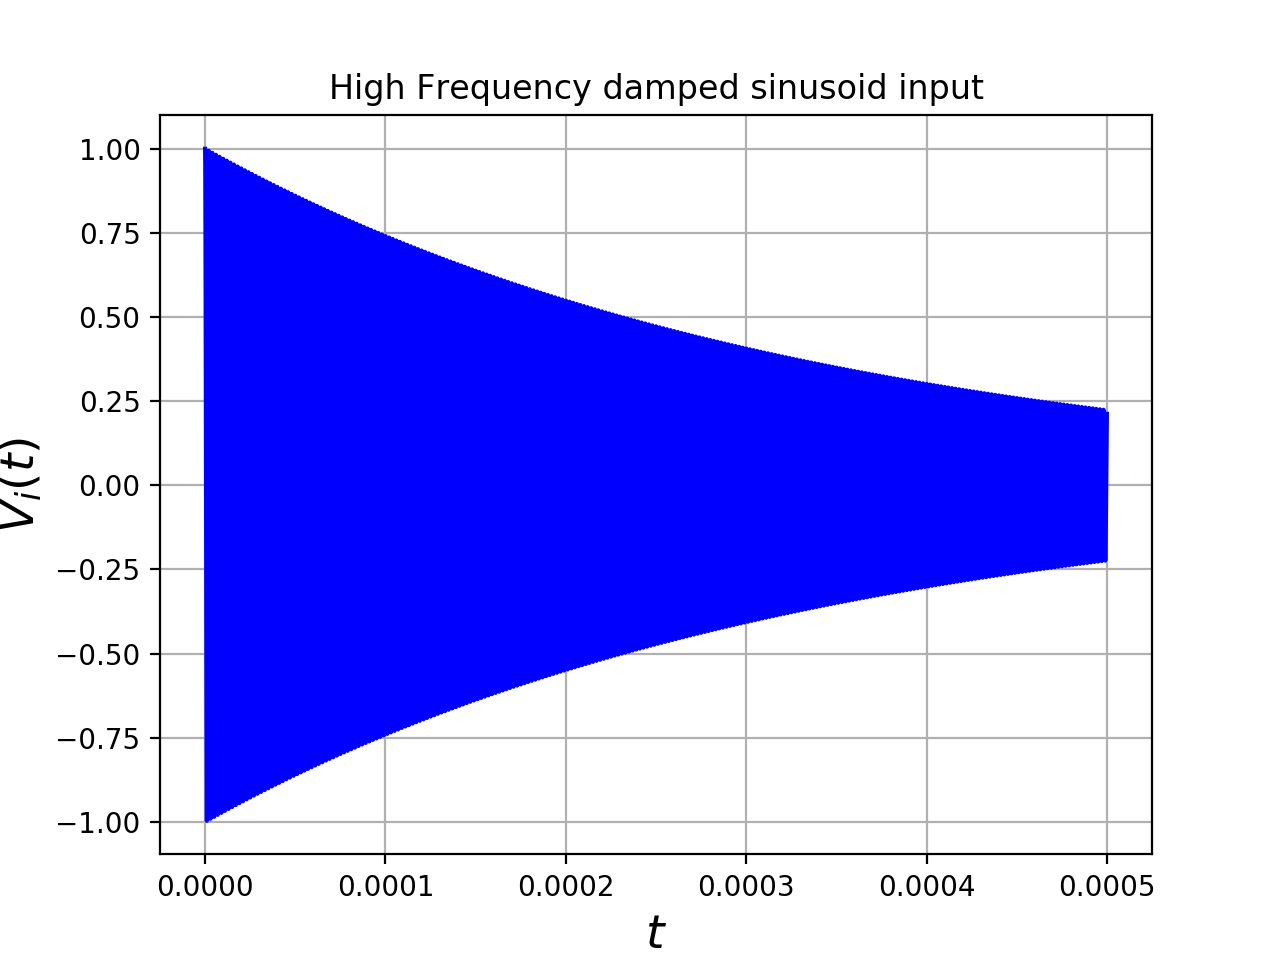
\includegraphics[scale=0.5]{vi_high.png}
   	\label{fig:vi_high}
   	\caption{Input damped sinusoid voltage of high frequency}
\end{figure}
\begin{figure}[H]
   	\centering
   	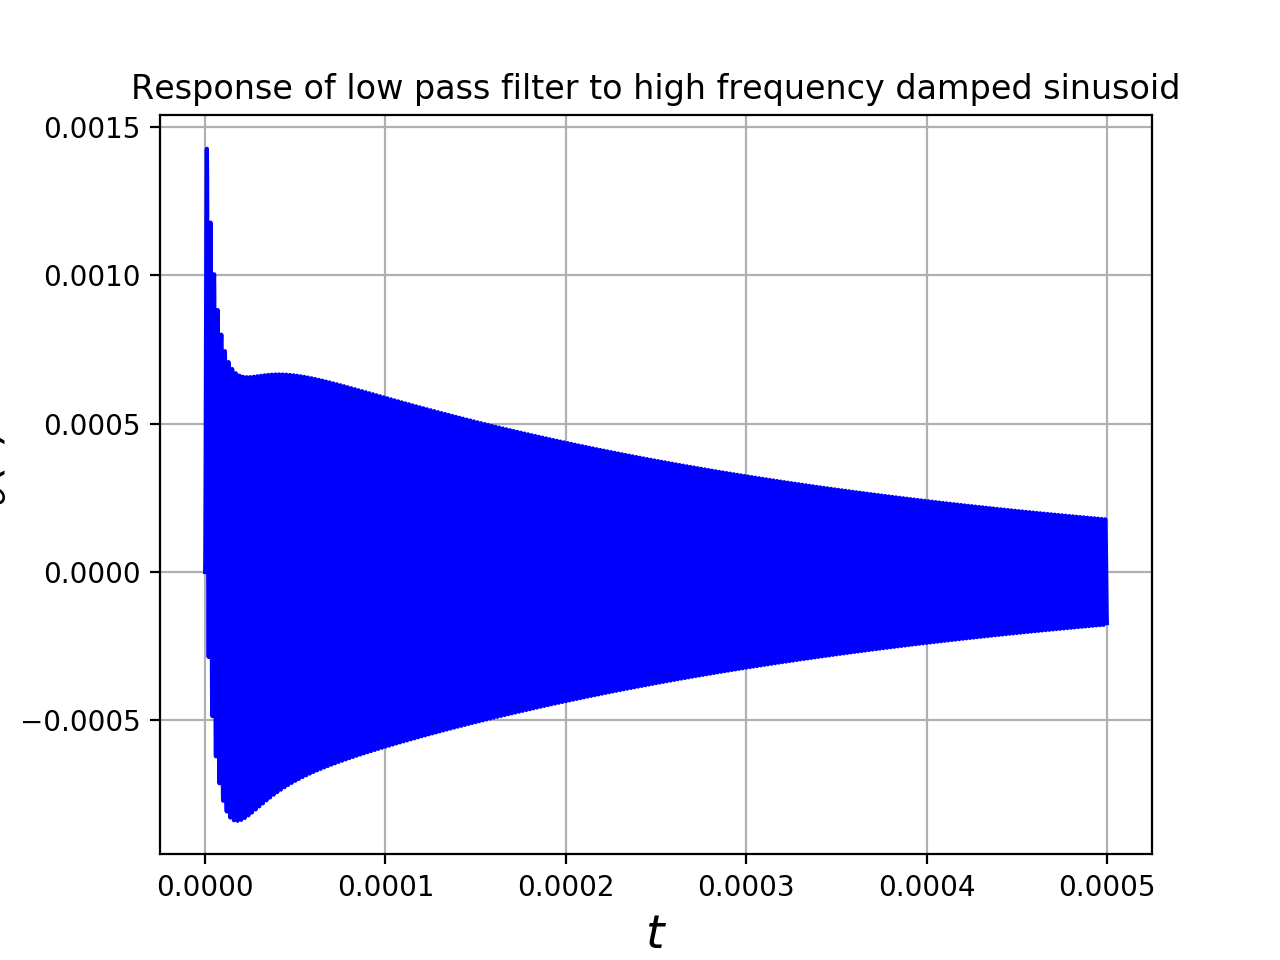
\includegraphics[scale=0.5]{lpf_high.png}
   	\label{fig:lpf_high}
   	\caption{Response of Low pass Filter to high frequency damped sinusoid}
\end{figure}
\begin{figure}[H]
   	\centering
   	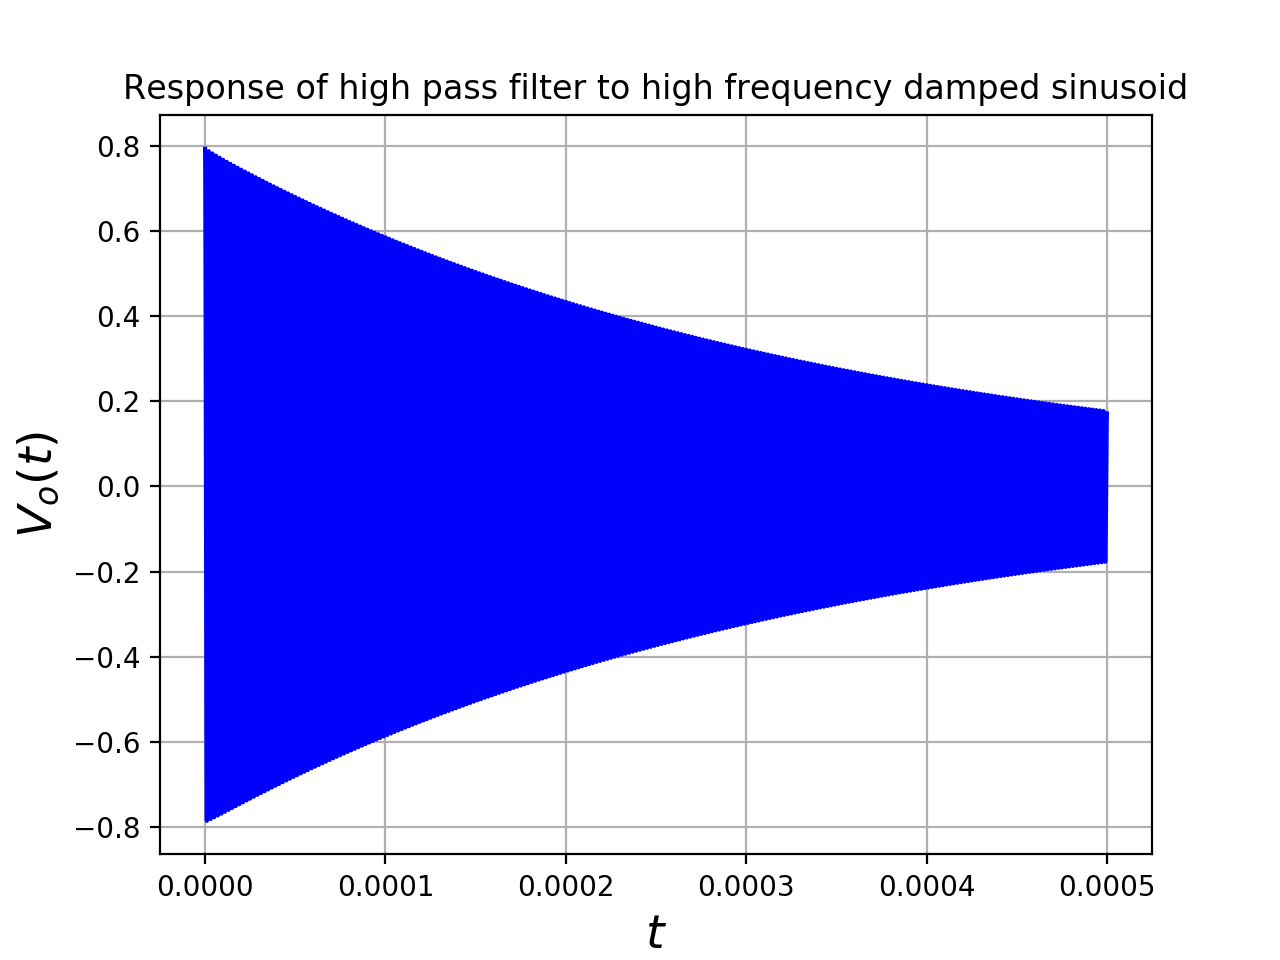
\includegraphics[scale=0.5]{hpf_high.png}
   	\label{fig:hpf_high}
   	\caption{Response of High pass Filter to high frequency damped sinusoid}
\end{figure}

\subsubsection{Low Frequency Damped sinusoid}
{
The second input voltage is given as :
\[v_i(t) = (\sin(10^3 t) \times e^{-100t})u(t)\]
}
\begin{minted}[obeytabs,tabsize = 4]{python3}
#Response of Low Pass and High Pass filter to low damped sinusoid
damping_factor = 100

t = np.arange(0,5e-2,1e-7)  #Time scale

inp = np.exp(-damping_factor*t)*(np.sin(1000*np.pi*t))
PLOT(t,inp,11,r'$t$',r'$V_i(t)$',title = 'Low Frequency damped sinusoid input')
pl.show()

t,vtd,svec = sp.lsim(H_lp,inp,t)
PLOT(t,vtd,12,r"$t$",r'$V_o(t)$',pl.plot,
	title = 'Response of low pass filter to low frequency damped sinusoid')
pl.show()

t,vtd,svec = sp.lsim(H_hp,inp,t)
PLOT(t,vtd,13,r"$t$",r'$V_o(t)$',pl.plot,
	title = 'Response of high pass filter to low frequency damped sinusoid')
pl.show()

\end{minted}
\begin{figure}[H]
   	\centering
   	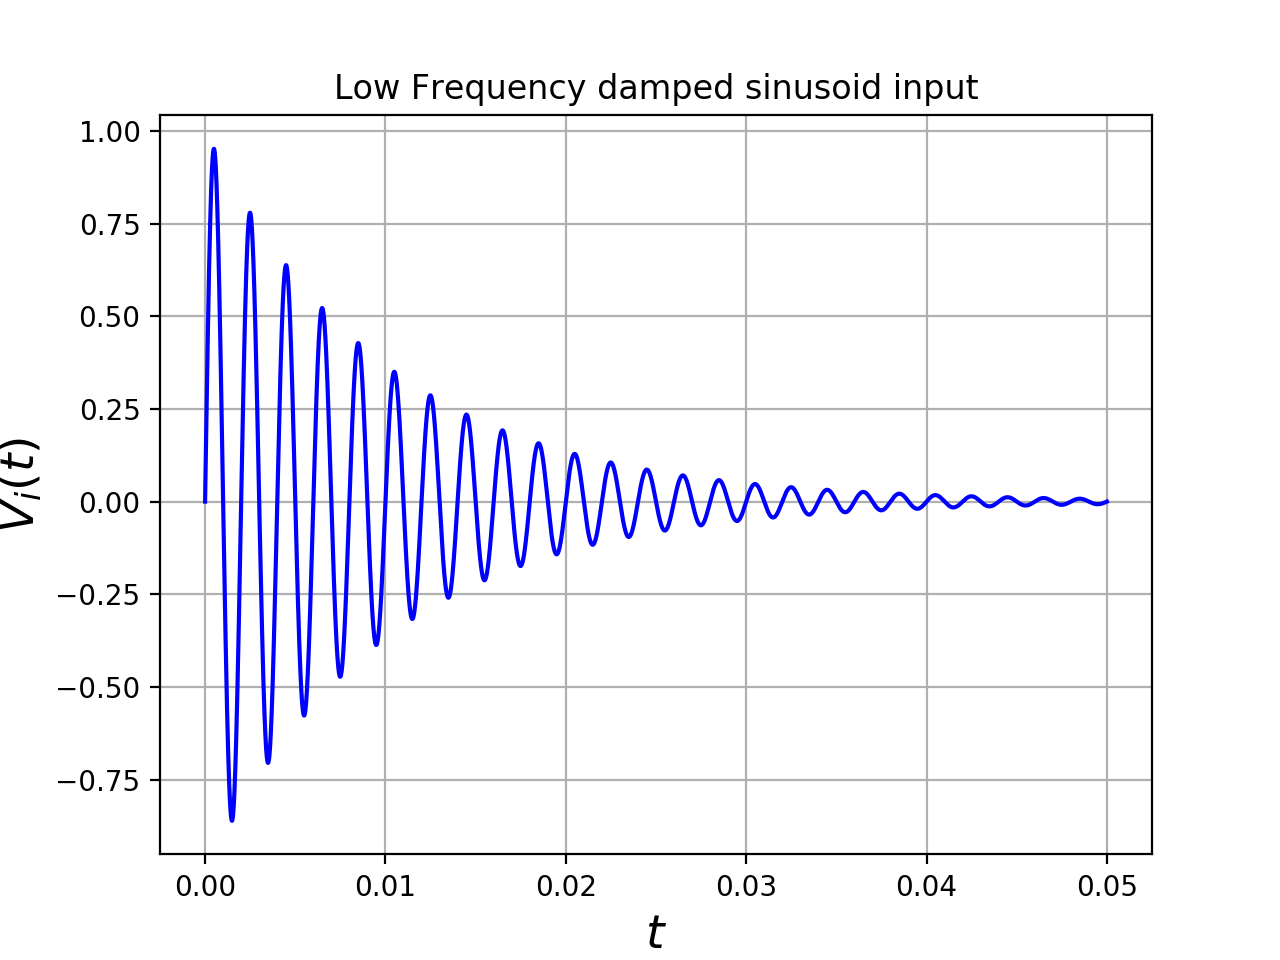
\includegraphics[scale=0.5]{vi_low.png}
   	\label{fig:vi_low}
   	\caption{Input damped sinusoid voltage of low frequency}
\end{figure}
\begin{figure}[H]
   	\centering
   	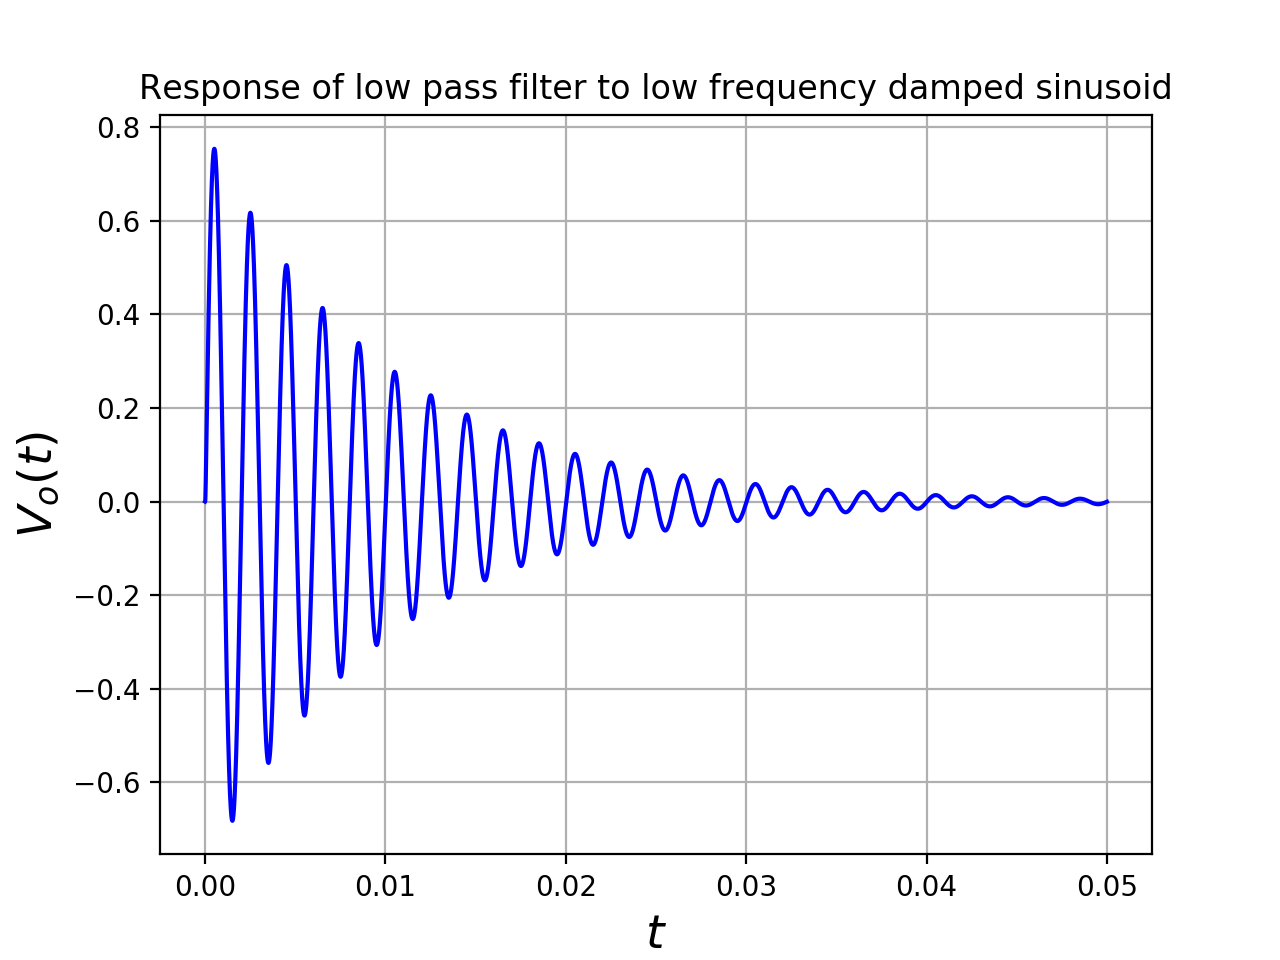
\includegraphics[scale=0.5]{lpf_low.png}
   	\label{fig:lpf_low}
   	\caption{Response of Low pass Filter to low frequency damped sinusoid}
\end{figure}
\begin{figure}[H]
   	\centering
   	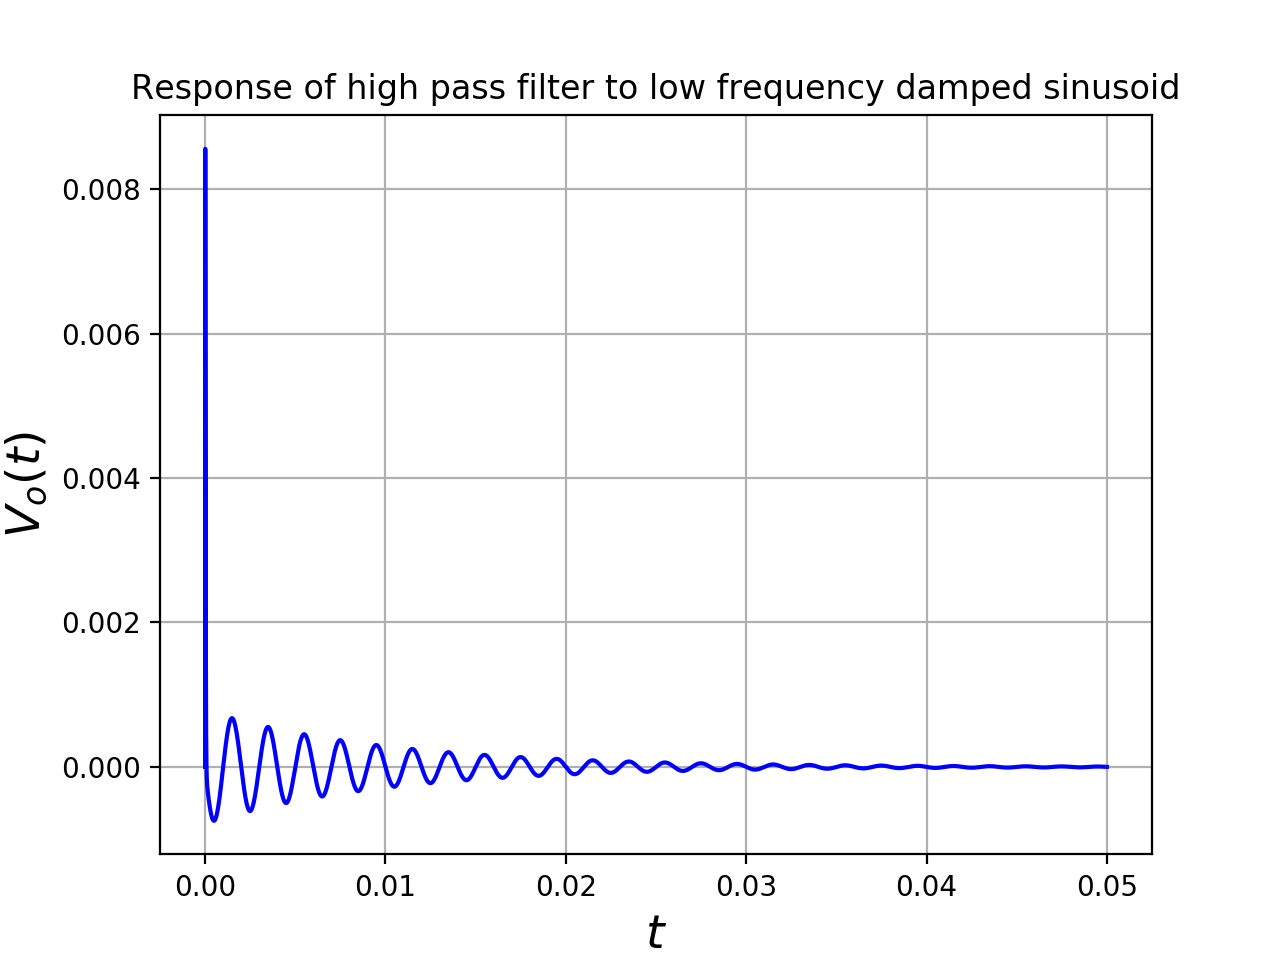
\includegraphics[scale=0.5]{hpf_low.png}
   	\label{fig:hpf_low}
   	\caption{Response of High pass Filter to low frequency damped sinusoid}
\end{figure}
{
We could observe how the \textbf{low pass filter nearly blocked the high frequency damped sinusoid} input (notice the low amplitudes and faster decay), and \textbf{almost perfectly allowed low frequency damped sinusoid} to pass through.
\\The opposite is observed for the high pass filter, where \textbf{in case of low frequency damped sinusoid there is initially a spike} due to sudden input given at t = 0 (hence high frequency), then the input decays very fast and hence is said to be \textbf{nearly blocked}. Whereas the \textbf{high frequency damped sinusoid is almost perfectly allowed}.
}

\subsection{Question 5}
{
We plot the \textbf{step response of High Pass Filter}, (i.e) output of high pass filter for input :
\(v_i(t) = u(t)\)
which implies $V_i(S) = 1/S$.
}
\begin{minted}[obeytabs,tabsize = 4]{python3}
t = np.arange(0,1e-2,1e-7)  #Time scale

A,b,V = HighPass(1e4,1e4,1e-9,1e-9,1.586,1/s)
_,vtd = sp.impulse(Simplify_H(V),None,t)
PLOT(t,vtd,4,r"$t$",r'$V_o(t)$',pl.plot,
	title = 'Step response of High Pass Filter')
pl.show()

\end{minted}
\begin{figure}[H]
   	\centering
   	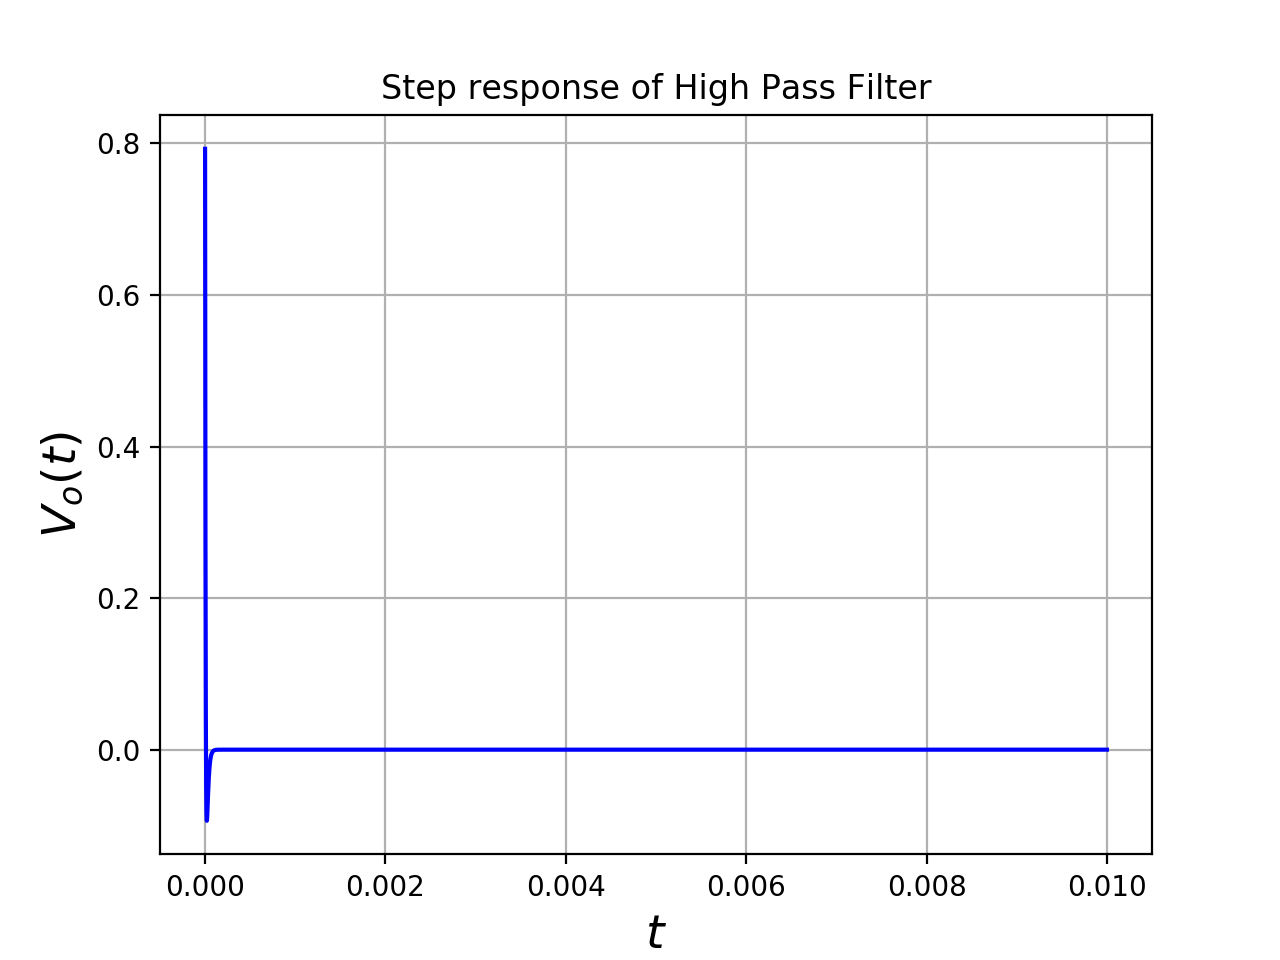
\includegraphics[scale=0.5]{step_hpf.png}
   	\label{fig:step_hpf}
   	\caption{Response of High pass Filter to unit step function}
\end{figure}
{ 
The high pass filter\textbf{ initially has a momentary high value} of 0.79 at t = 0 because of sudden input given (high frequency) which is allowed by it.
\\It then becomes zero, showing it \textbf{doesn't allow low frequency DC} input to pass through.
\\\textbf{Overshoot} is observed in case of high pass filter.
}

\section{Conclusions}
\begin{itemize}
\item We  solved Laplace equations in 's' using sympy in Python.
\item We analysed and solved opamp circuits using sympy, and realised low pass and high pass filters using the same.
\item We made Bode plots, and plotted step responses and sinusoidal responses to understand the behaviour of low pass and high pass filters.
\end{itemize}

\end{document}